\documentclass[../../../../main.tex]{subfiles}
\begin{document}

\begin{flushright}
\footnotesize\textit{【自動文字起こし・要確認】}
\end{flushright}

[解] ABと$y$軸の交点Cとすると、対称性から
\[
(\Delta \text{PAB}) = 2(\Delta \text{PAC}) \cdots \text{①}
\]
である。双曲線上の点 $(X, Y)$ ($0<X$) での接線は
\[
Xx - Yy = 1 \cdots \text{②}
\]

\begin{center}
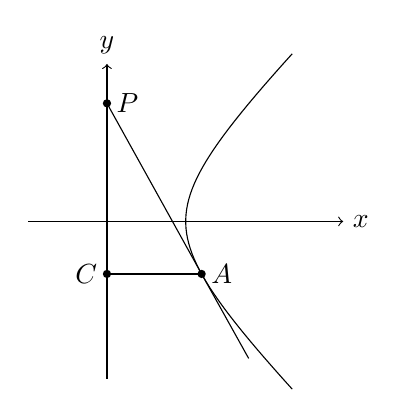
\begin{tikzpicture}
\draw[->] (-1,0) -- (3,0) node[right] {$x$};
\draw[->] (0,-2) -- (0,2) node[above] {$y$};
\draw[domain=-1.5:1.5, samples=50, variable=\t] plot ({cosh(\t)}, {sinh(\t)});
\coordinate (P) at (0, 1.5);
\node[right] at (P) {$P$};
\fill (P) circle (1.5pt);
\coordinate (A) at ({sqrt(1+(-1/1.5)^2)}, {-1/1.5});
\node[right] at (A) {$A$};
\fill (A) circle (1.5pt);
\coordinate (C) at (0, {-1/1.5});
\node[left] at (C) {$C$};
\fill (C) circle (1.5pt);
\draw (P) -- (A) -- (1.8, -1.74);
\draw (C) -- (A);
\end{tikzpicture}
\end{center}

これが $P$ をとおる時、
\[
-Yp = 1 \cdots \text{③}
\]
$\Delta \text{PAC}$ の面積 $S(p)$ とすると
\[
S(p) = \frac{1}{2}X \cdot (p-Y) \cdots \text{④}
\]
③と $p>0$ から $Y = -\frac{1}{p}$ だから、$X^2-Y^2=1$ に代入 ($X>0$)
\[
X = \sqrt{1+Y^2} = \sqrt{1+\frac{1}{p^2}}
\]
以上を④に代入
\begin{align*}
S(p) &= \frac{1}{2} \cdot \frac{\sqrt{p^2+1}}{p}\left(p+\frac{1}{p}\right) \\
&= \frac{1}{2} \sqrt{\frac{(p^2+1)^3}{p^4}}
\end{align*}
$\sqrt{\quad}$ の中を $f(p)$ とおくと、$f(p)$ が $\min$ の時、$S(p)$ が $\min$ で、①から $\Delta \text{PAB}$ の面積も $\min$ となる。
\begin{align*}
f(p) &= \frac{t^3}{(t-1)^2} \quad (t=p^2+1, t>1) \\
&= \frac{1}{\alpha^3-2\alpha^2+\alpha} \quad \left(\alpha=\frac{1}{t}, 0<\alpha<1\right)
\end{align*}
分母を $g(\alpha)$ とおくと
\[
g'(\alpha) = 3\alpha^2-4\alpha+1 = (\alpha-1)(3\alpha-1)
\]
より、下表をえる

\begin{center}
\begin{tabular}{|c|c|c|c|c|c|}
\hline
$\alpha$ & $0$ & $\cdots$ & $1/3$ & $\cdots$ & $1$ \\
\hline
$g'$ & & $+$ & $0$ & $-$ & \\
\hline
$g$ & & $\nearrow$ & & $\searrow$ & \\
\hline
\end{tabular}
\end{center}
よって $\alpha = \frac{1}{3}$ の時、$f(p)$ は $\min$ である。この時 $\alpha = \frac{1}{p^2+1}, p>0$ から $p = \sqrt{2}$

\textcolor{cyan}{[本時のミス]}\\
\textcolor{cyan}{次数をまちがえ}

\end{document}
